%!TEX root = gorila_paper.tex

\section {Results}

\begin{figure}[ht]
	\vskip -0.1in
	\begin{center}
		\centerline{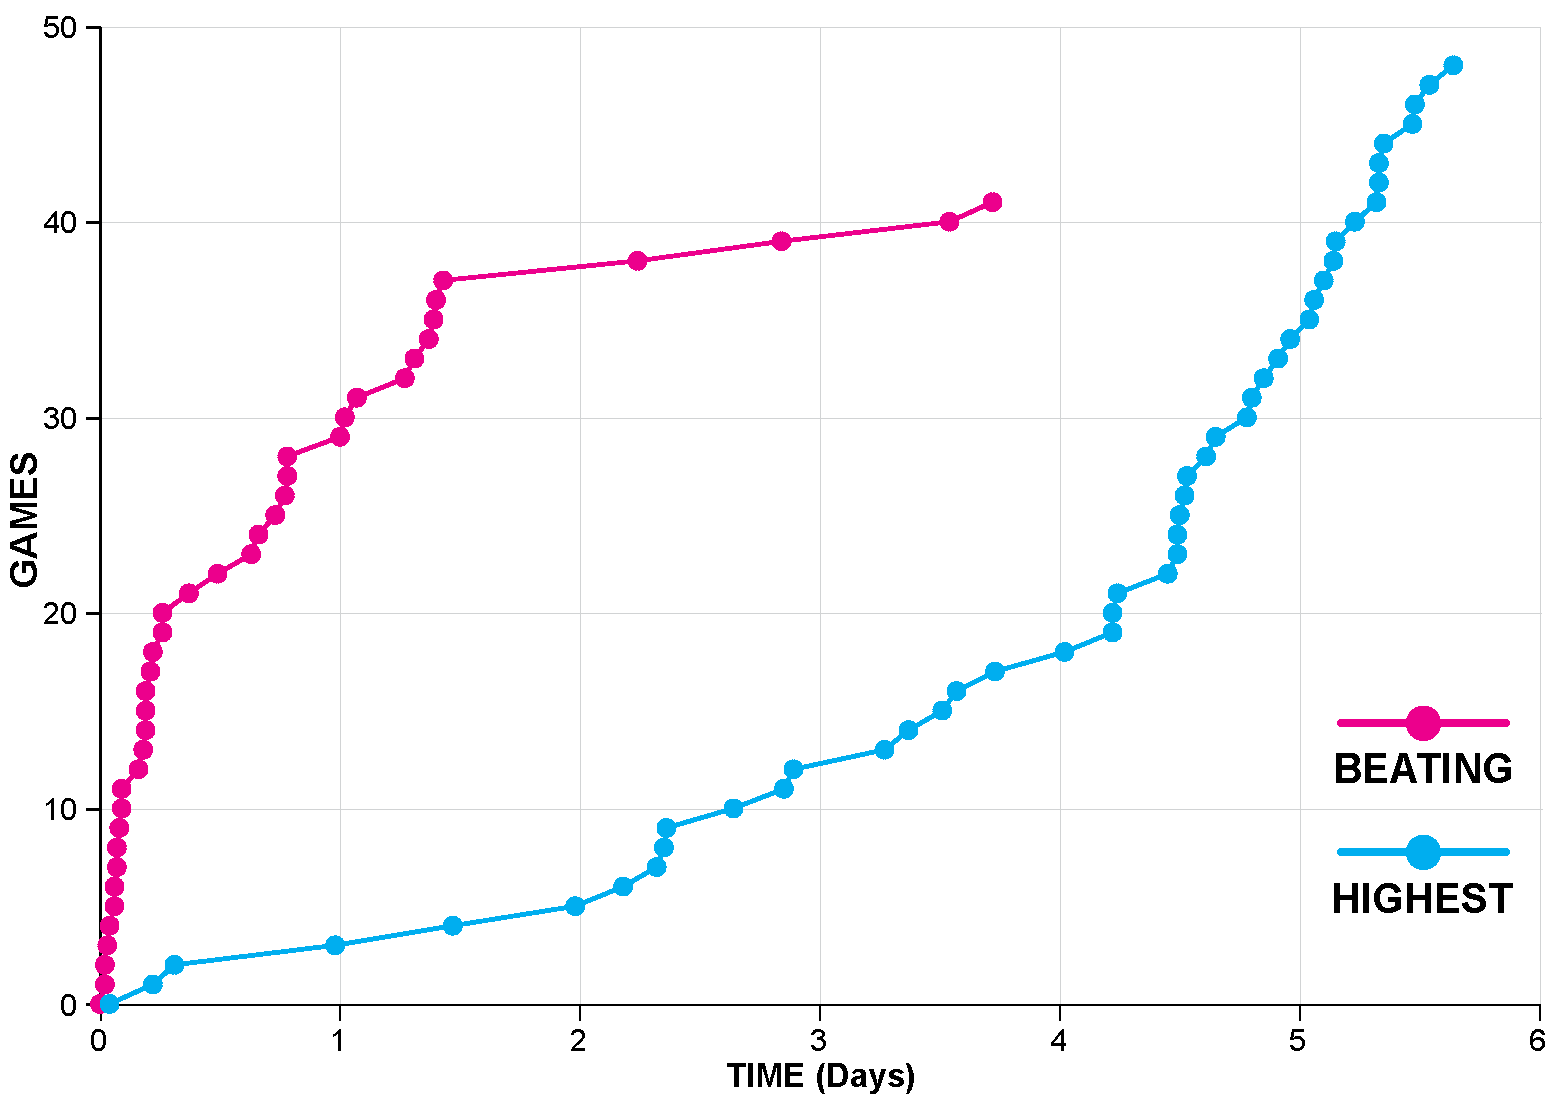
\includegraphics[width=\columnwidth]{TimeGraph3}}
		\caption{
			The time required by Gorila DQN to surpass single DQN performance (red curve) and to reach its peak performance (blue curve). 
		}
		\label{fig:time}
	\end{center}
	\vskip -0.2in
\end{figure}

We first compared Gorila DQN agents trained for up to 6 days to single GPU DQN agents trained for 12-14 days.
Figure~\ref{fig:humanstarts} shows the normalized scores under the human starts evaluation.
Using human starts Gorila DQN outperformed single GPU DQN on 41 out of 49 games given roughly one half of the training time of single GPU DQN.
On 22 of the games Gorila DQN obtained double the score of single GPU DQN, and on 11 games Gorila DQN's score was 5 times higher.
Similarly, using the original {\it null op starts} evaluation  Gorila DQN outperformed the single GPU DQN on 31 out of 49 games. 
These results show that parallel training significantly improved performance in less training time. Also, better results on {\it human starts} compared to {\it null op starts} suggest that Gorila DQN is especially good at generalizing to potentially unseen states compared to single GPU DQN.  Figure~\ref{fig:humanstarts1} further illustrates these improvements in generalization by showing Gorila DQN scores with human starts normalized with respect to GPU DQN scores with human starts (blue bars) and Gorila DQN scores from null op starts normalized by GPU DQN scores from null op starts (gray bars).
In fact, Gorila DQN performs at a level similar or superior to a human professional (75\% of the human score or above) in 25 games despite starting from states sampled from human play.
One possible reason for the improved generalization is the significant increase in the number of states Gorila DQN sees by using 100 parallel actors.


We next look at how the performance of Gorila DQN improved during training.
Figure~\ref{fig:time} shows how quickly Gorila DQN reached the performance of single GPU DQN and how quickly Gorila DQN reached its own best score under the human starts evaluation.
Gorila DQN surpassed the best single GPU DQN scores on 19 games in 6 hours, 23 games in 12 hours, 30 in 24 hours and 38 games in 36 hours (red curve).
This is a roughly an order of magnitude reduction in training time required to reach the single process DQN score.
On some games Gorila DQN achieved its best score in under two days but for most of the games the performance keeps improving with longer training time (blue curve).


